A streaming transcript can arrive on time and still disappear when trusted
feedback advances. In one actual run, a complete two-second audio interval
introduced 37 visible characters at 1.444~s, within its two-second display
deadline. A trusted update at 1.544~s replaced that whole hypothesis with
a shorter snapshot, although its computation remained compatible with the
selected feedback state. Identical text returned through certified
delivery at 3.720~s, within the eight-second deadline. Both first-delivery
obligations were met, yet the phrase was absent for 2.176~s, including at
the original display deadline (Figure~\ref{fig:continuity_case}). The
service lost delivered progress without needing to correct it. Trusted
feedback here means feedback accepted by protected selection.

\begin{figure*}[t]
\centering
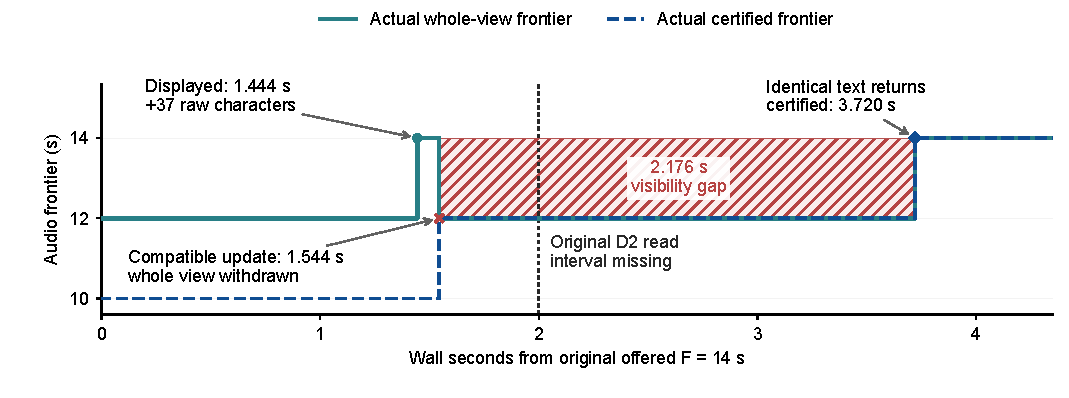
\includegraphics[width=\textwidth]{figures/timely_full_interval_case.pdf}
\caption{Timely first delivery can still leave a gap in delivered progress.
An actual computation-only run displays a complete interval at 1.444~s,
withdraws it under a compatible update at 1.544~s, and restores identical
text at 3.720~s. Shading marks the 2.176-s gap; the vertical line is the
original D2 read point. The view introduces 37 raw code points including
spaces, not character/audio alignments. This c16 overload case illustrates
the failure mode, not its incidence or a whole-run service win.}
\label{fig:continuity_case}
\end{figure*}

This problem arises when generated or corrected output becomes an input
to subsequent inference. Streaming speech correction is a concrete case:
StreamCorrect feeds its chosen correction into later recognition
\cite{vu2026streamcorrect}. A new trusted selection can invalidate some
speculation while confirming other work that began earlier. Recomputing
everything is conservative, but retaining computation alone is also
insufficient. In our predeclared 24-speaker evaluation, computation
retention improves timely delivery while increasing audio-frontier
withdrawals from 12 to 17. Jointly retaining computation and its supported
whole view yields zero. The missing obligation is to turn valid work into
\emph{sustained service} across a trusted revision.

Three questions determine the actions. Does an old call's complete frozen
input still match the selected parent feedback state? Has the original selection
authorized its result? Does the Consumer's current whole hypothesis still
have a complete dependency path from that parent? These questions concern
different objects. A call can have a confirmed input while its own next
prediction is wrong. A view can lose support while a future call's input
is unresolved. A producer can die after its complete result has already
been accepted. A birth version, matching text, or producer-liveness bit
cannot stand in for all three judgments.

RevTrace checks complete frozen inputs and dependency paths before
retaining work, leaves result selection to the original program, and
revalidates the Consumer's entire displayed hypothesis when a selected
state installs.
Incremental dialogue and computation supply established dependency and
revocation principles~\cite{schlangen2011incremental,hammer2014adapton,hammer2015names}.
SSBD already combines draft reuse and display masking
\cite{zeng2026ssbd}; PredGen speculates across evolving speech stages
\cite{li2025predgen}. Our focus is a recursively selected feedback task:
retained work must still execute its original correction and update, and
applying a new selected root must separately validate the actual whole
view. The contribution is this concrete coordination contract and its
service consequences, rather than reuse or revocation in isolation.

We make three contributions:
\begin{itemize}
\item We identify a service gap between timely first delivery and continued
  availability under compatible feedback, and define executable witnesses
  for complete-call eligibility and whole-view retention
  (Sections~\ref{sec:contract}--\ref{sec:continuation}).
\item We implement their joint coordination with original selection,
  durable facts, and physical ownership. A conditional selected-trace
  refinement argument explains how early full calls preserve the protected
  task, including accepted results across supported process failures
  (Sections~\ref{sec:continuation}--\ref{sec:protocol}).
\item We test the composition on real neural service: factorial controls
  isolate the interaction, native correction tests original full calls,
  and fault and sustained-state controls establish its costs and limits
  (Section~\ref{sec:eval}).
\end{itemize}

Deadline credit counts offered audio seconds meeting both first-display
and certified-delivery deadlines. The headline joint arm adds 26.645~s over
714.110~s offered with unchanged selected histories. A matched native
comparison raises credit from 30.0 to 65.822 of 66.340~s and whole-run
passes from zero to six of eight; resident independent requests pass
seven of eight. The remaining EOS misses, overload, cold recovery, and
no-reset quality failures delimit the service claim.
